\documentclass[aps,twocolumn,floatfix,prl,10pt]{revtex4-1}
%\documentclass[letterpaper,10pt,prl,twocolumn,aps]{revtex4-1}
%\documentclass[aps,preprint,floatfix,prl]{revtex4-1}
\usepackage{fullpage}
\usepackage{amsmath}
\usepackage{amsfonts}
\usepackage{amssymb}
\usepackage{graphicx}
\usepackage{slashbox}
\usepackage{color}
\usepackage{longtable}
\usepackage{array}
\usepackage{dashrule}
\usepackage{amsmath}

\usepackage{dcolumn}% Align table columns on decimal point

\usepackage{graphicx}% Include figure files
\usepackage{dcolumn}% Align table columns on decimal point
\usepackage{bm}% bold math
\usepackage{ifthen}
\usepackage{amsthm} % Theorem Formatting
\usepackage{amssymb}	% Math symbols such as \mathbb
\usepackage{calrsfs}
\graphicspath{ {images/} }

\newcommand{\ellcap}{{\ell_\text{c}}}
\newcommand{\Fh}{{\boldsymbol{F}_h}}
\newcommand{\Fv}{{\boldsymbol{F}_v}}
\newcommand{\Tv}{{\boldsymbol{T}}}
\newcommand{\bn}{{\boldsymbol{n}}}
\newcommand{\bt}{{\boldsymbol{t}}}
\newcommand{\bz}{{\boldsymbol{z}}}
\newcommand{\bx}{{\boldsymbol{x}}}
\newcommand{\by}{{\boldsymbol{y}}}
\newcommand{\bT}{{\boldsymbol{T}}}
\newcommand{\bu}{\mathbf{u}}
\newcommand{\grad}{\mathbf{\nabla}}
\newcommand{\del}{\partial}

\begin{document}
\title{Waving and swaying}
\author{Ravi Singh, Shreyas Mandre}
\affiliation{Brown University, Providence RI 02912 USA}
\author{L. Mahadevan}
\affiliation{Harvard University, Cambridge MA 02138 USA}
\author{Mahesh Bandi\footnote{work performed while visiting Brown University}}
\affiliation{Okinawa Institute of Science and Technology, Okinawa, Japan}
\author{Amala Mahadevan}
\affiliation{Woods Hold Institute of Oceanography, Woods Hole MA USA}
%\author{Shreyas Mandre}
%\affiliation{Brown University, Providence RI 02912 USA}

\begin{abstract}
The spontaneous waving of marine grass is thought to be due to a Kelvin-Helmholtz instability resulting from an inflection point in the flow profile. 
We find that this inflection point is located inside the grass canopy but it does not lead to Kelvin Helmholtz instability which is 
normally observed in a free shear layer. We also show that the wavelength of coherent vortices scales with the unvegetated water depth, and not with 
the shear layer thickness as predicted by a theory based on Kelvin-Helmholtz instability. Based on these results, we propose a mechanism for waving 
marine grass based on the shear instability of the flow above the canopy.

%The spontaneous waving of marine grass is though to be due to a Kelving-helmholtz instability resulting from strong shear near top of grass. On the contrary
%we find that strong velocity shear resulting from vertical discontinuity of drag due to presence of grass does not lead to Kelvin-Helmholtz instability which is 
%normally observed in free shear flows. We also show that wavelength of coherent vortices scales with the unvegetated water depth. Based on these results, 
%we propose an alternative mechanism which attributes waving of marine grass on shear instability of flow above the canopy. 
\end{abstract}
\maketitle

\section{Introduction}
Sea grasses exhibit rich set of dynamics due to their interaction with the flow of water and can considerably affect surrounding hydrodynamic conditions.
Resulting changes in hydrodynamic conditions can influence number of environmental variables and processes such as 
transport of sediments, contaminants, dissolved oxygen, plant growth and biomass production etc. 
The response of flexible grass canopies to steady current in form of large amplitude coherent oscillation, known as mo-nami (Ackerman and Okubo, 1993), plays a central role
in the recruitment of microscopic marine organism such as blue mussel larvae. The hydrodynamic mechanism underlying monami is the focus of this paper. 
\newline
Similar phenomenon of large amplitude coherent oscillation of canopy in wind known as ho-nami (Inoue 1955, Raupach 1996) have also been observed.
A crucial difference between the atmospheric and aquatic flow is that the atmospheric flows are essentially unbounded vertically. Another major
difference between the two is the considerable difference of stiffness of canopies; terrestrial canopies tend to be much more rigid than aquatic canopies.
Due to these considerable differences between aquatic and marine flow the analysis in this paper is applicable only to marine canopies  
\newline   
Existing explanation of mo-nami invokes the existence of strong shear near the top of the canopy (Ghisalberti 2002, Raupach 1996) due to
different amounts of drag experienced by fluid in and above the canopy. This shear layer is assumed to become unstable to coherent vortices through a mechanism similar to Kelvin-Helmholtz
instability. Influence of these coherent eddies over sea grasses is manifested in their large amplitude synchronous oscillations.
%Sea grasses exhibit large amplitude wave like motion in response to these eddies propagating downstream.
%are exhibited in form of large amplitude oscillations knows as mo-nami.
\newline
While shear layer model successfully predict frequency of mo-nami for number of experimental observations,
several aspect of existing theory remain unexplained. First, linear stability analysis of base flow does not take into account influence of drag due to grass hence not a self consistent 
theory. Second, classical free shear flow is known to be unstable above a very small Reynolds number $\leq 10 $. On the contrary observed critical Reynolds number (Grizzle 1996) 
for monami is much higher $\approx O(1000)$. These drawbacks of existing theory suggest that flow through vegetation requires further investigation for better understanding of
phenomenon.
\newline 
In this paper we extend the idea of Raupach et.al via incorporating drag due to presence of vegetation. Our calculation of linear stability analysis of flow in presence of grasses 
shows that existence of strong shear near canopy top does not lead to Kelvin Helmholtz instability. We also show instead that mo-nami is caused by instability 
of fluid flow above vegetation coupled with the flow through canopy. We further show that inclusion of drag due to grass predicts a threshold condition for waving where threshold is
characterized by Reynolds number. We confirm our analysis by comparing prediction from theory with field and experimental observations.  
%\section{The model}
%Monami is believed to be response to strong oscillations of flow in streamwise velocity associated with coherent vortices.
\newline
While Drag exerted by canopy is believed to play 
a significant role in the development of coherent vortices leading to monami, flexibility of grass provide striking visualization of these structures without significantly affecting the
dynamics of flow (Raupach 1996, Ghisalberti 2002). For this reason we replace grass with stiff structure to investigate dynamics leading to generation of 
coherent vortices. We use a mean field model for the coupling between the flow and the canopy. 
%The drag force per unit volume experienced by fluid flow is believed to be dependent on
%mean frontal area of grass. We approximate mean frontal area of grass field of height $h$ with $dN_g/m^2$. Where $d$ is average width of grass and $N_g$ the grass number density per unit area 
Drag force exerted by the grass is approximated via a continuous body force $\mathbf{f}=-N_g\mathbf{f_d}$ in the fluid momentum balance as
%We propose a fully coupled model in order to comprehend dynamics of canopy and fluid flow, drag force excerted by grasses is
%taken as an additional body force in momentum equation of fluid. We approximate presence of grass via continuous field whose shape at any location is approximated as averaged 
%shape of grass at that location which can be obtained by assuming grass to be in quasi-equilibrium at any moment.
% and solving force balance and momentum balance for grass  
\begin{equation}
\rho \left(\bu_{t}+\bu.\grad\bu \right) = -\grad P+\mu\grad^{2}\bu +\mathbf{f}+\rho\mathbf{g}
\end{equation}
%\begin{equation}
% \mathbf{f}=-N\mathbf{f_{d}}
%\end{equation}
where $\mathbf{f_{d}}$ is drag force per unit length of the grass blade, $N_g$ the grass number density per unit area, $\rho$ the fluid density, $\mathbf{u}$ the velocity, 
$P$ the pressure, $\mu$ the viscosity and $\mathbf{g}$ the acceleration due to gravity. Drag force itself is modeled 
as $\mathbf{f_{d}}=C_N \rho u_{N}^{2}d\hat{n}+C_{T}\rho u_{T}^{2}d\hat{t}$ where $d$ is average width of grass blade 
$C_{N}$ and $C_{T}$ are normal and tangential drag coefficients respectively which are set to zero outside the grass; $\bu_{T}$, $\bu_{N}$ are velocity vector along and
normal to grass while $\hat{t},\hat{n}$ being unit vector along and normal to grass. We expect $C_T \ll C_N$ and take $C_T=0$ for rest of analysis. We further expect $C_N$ to
not change along the height of the grass and take $C_N$ to be constant. 
%\begin{equation}
% \mathbf{f_{d}}=C_N \rho\bu_{N}^{2}d\hat{n}+C_{T}\rho\bu_{T}^{2}d\hat{t}
%\end{equation}\
%\begin{equation}
%\begin{split}
% \frac{\del}{\del s}\left(T\hat{t}+N\hat{n}\right) & +\mathbf{f_{d}}+\mathbf{f_{buoy}} = 0\\
% \frac{\del M}{\del s}&-N = 0\\
% M &= B\kappa
%\end{split}
%\end{equation}
%where $C_{N}$ and $C_{T}$ are normal and tangential drag coefficients respectively; $\bu_{T}$, $\bu_{N}$ are velocity vector along and normal to grass.
%\section{Stability Analysis}
\newline
A solution of equation(1) gives uniform steady flow which we expect to be unstable leading to generate coherent eddies. To understand the instability characteristic associated with this
steady flow termed as base flow we perform linear stability analysis.  
%We perform linear stability analysis of a base state associated with the vegetated flow to gain insight about instability characteristics of flow in presence of grass.
This base state flow is obtained by solving steady state form of constant pressure gradient driven flow of equation(1)
$-\frac{dP}{dx}+\mu\frac{d^2U}{dy^2}+\rho C_N d N_gU^2=0$ with no slip at bottom and zero shear at top of surface Fig(1). Flow consist of a region of approximately constant velocity
$U_g \sim \sqrt{\frac{dP/dx}{\rho C_N dN_g}}$ arising from balance of drag force with pressure gradient with in grass and a parabolic velocity profile in unvegetated region due to 
balance of viscous force and pressure gradient. No slip condition at bottom and continuity of shear stress at canopy top give rise to two boundary layer in the flow profile one 
near bottom and near the tip of the grass which is conventionally known as shear layer.
%eads to a 
%constant velocity $U_g \sim \sqrt{\frac{dP/dx}{\rho C_N dN_g}}$ while balance of viscous force with pressure gradient above grass provide a parabolic velocity profile.
%The base flow profile consist of two boundary layer one near the bottom of grass due to no slip condition and other near tip of canopy known as shear layer due to vertical discontinuity 
%of drag force. Width of boundary layer near bottom of grass can be obtained by balance of viscous force with drag and pressure gradient forces which gives boundary layer
%width $\sim \sqrt{\frac{\mu}{\rho C_NdN_g U_g}}$. 
Thickness of shear layer near top of grass is obtained by balance of viscous force 
with drag along with match of shear at grass tip exerted by flow in unvegetated region, which leads to shear layer 
width $\delta \sim  H\left(\frac{\rho U_0 H}{\mu} C_N d N_g H\right)^{-1/3}$ where $U_0 = \frac{dP/dxH^2}{\mu}$ is scale for velocity.
 
\begin{figure}[htb!]
  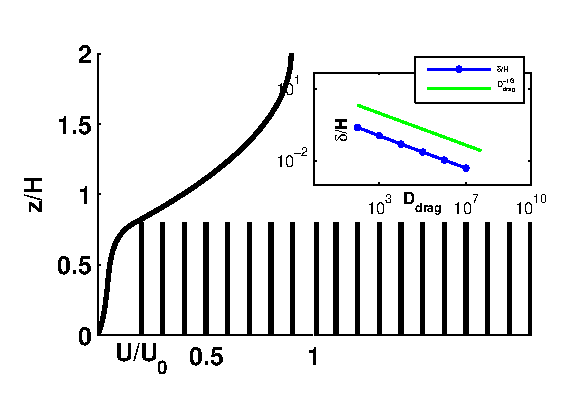
\includegraphics[]{fig1}
\caption{Basic flow profile (left )and model of canopy (bottom) along with variation of shear layer (inset) }
\end{figure}
Knowing the scale of shear layer we can systematically investigate its effect on flow instability
by varying grass number density $N_g$ and pressure gradient $\frac{dP}{dx}$. Considering small perturbations $u, v, p$ about the base profile $U$ and $P$
respectively, momentum and mass balance equation expanded in first order of perturbed variable yields.
\begin{equation}
%\scriptstyle{
\begin{split}
 %u_t+Uu_x+vU_y &= \frac{1}{\rho}p_x+\frac{\mu}{\rho}\left(u_xx+u_yy \right) -2C_NdN_gUu\\
\frac{\del u}{\del t}+U\frac{\del u}{\del x}+v\frac{\del U}{\del y} &= -\frac{1}{\rho}\frac{\del p}{\del x}+\frac{\mu}{\rho}\nabla^2u-2C_{N}dN_{g}Uu\\
\frac{\del v}{\del  t}+ U\frac{\del v}{\del x} &= -\frac{1}{\rho}\frac{\del p}{\del y}+\frac{\mu}{\rho}\nabla^2v, \hspace{0.3cm} \nabla\cdot\bu=0\\
 %\nabla\cdot \bu &= 0
\end{split}
%}
\end{equation}
%In most of recent work on honami/monami base profile have been approximated to a plane mixing layer profile having inflection point near top of canopy, It is also argued that 
%It is instability associated with inflection of mean velocity which is responsible for coherent eddies traveling on top of canopies. In our calculation we get base velocity
%profile by hydrodynamic balance between pressure, drag and diffusive force which also results in a velocity profile with inflection point near top of canopy with additional property 
%of having been produced through equation of motion itself.\newline
%We performed stability analysis on two different kind of base flow namely (1) flow driven by constant pressure gradient between two parallel plate (2) constant pressure gradient driven 
%flow with zero shear at top. We use following scaling to non-dimensionlize equation of motion
Momentum and mass balance equation can be non-dimensionlize using half channel height $H$, associated advection time H/$U_0$ and velocity $U_0 = \frac{dP/dxH^2}{\mu0}$.
%Using half channel height $H$ of and associated advection time H/$U_{0}$, we use following scaling to non-dimensinlize equation 
%of motion
%   \[ u = U_{0}\bar{u},\hspace{1cm} y = (H/2)\bar{y}, \hspace{1cm} \text{with}\hspace{2mm} U_{0}=\frac{(dP/dx)H^2}{4\mu} \]
With these scaling along with the use of stream function $\psi$ with $u = \psi_{y}, v= -\psi_x$ to satisfy mass balance; momentum and mass balance can be combined 
into a single equation.
\begin{equation}
\scriptstyle{
Re\left[\del_t+\del_x U \right]\grad^2\psi - U_{yy}\psi_x = \grad^4\psi-\frac{\del}{\del_y}\left(\frac{2D_{drag}}{R_e}U\psi_y\right)
}
\end{equation}
where $R_{e}= \frac{\rho U_0 H}{\mu}$ is Reynolds number and $\bar{N_g} = C_N d N_g H$ is non-dimensional grass number density and  $D_{drag} = R_{e}\bar{N_{g}}$ is 
non-dimensional drag. Seeking wave solution in form of $\left(u,v,\psi \right)= \left(\hat u, \hat v, \hat\phi \right)e^{ikx+\sigma}$, we get generalized orr-sommerfield equation 
which is an eigenvalue problem whose solution provides frequency and wavelength of eddies traveling over canopy.
\begin{equation}
\begin{split}
\left(\sigma+ikU\right) \left(D^2-k^2\right)\phi &= \frac{1}{R_{e}}\left[D^2 -k^{2} \right]^2\phi +ikU_{yy}\phi \\
&-\frac{\del}{\del y}\left(\frac{2D_{drag}}{R_e}U\phi_y\right)
\end{split}
\end{equation}
Solution of generalized Orr-Somerfield equation predicts a critical Reynolds number as function of grass number density, below which there is no hydrodynamic instability (Fig(2))

% shows 
%this critical number for different grass density and grass height along with experimental threshold observed by Grizzle (1996)
  \begin{figure}[htb!]
  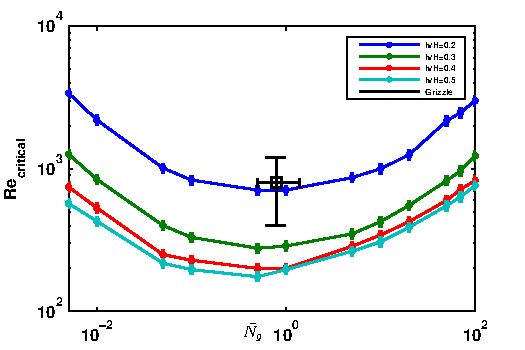
\includegraphics[]{Critical_Re_vs_Ng_Grizzle}
\caption{Critical Reynolds number with flow between parallel plate for different grass height as a function of grass number density}
\end{figure}


\end{document}
